\chapter{Resultados económicos: cartera, perfiles y confirmación reservada}
\label{chap:resultados-economicos}

El capítulo anterior cerró el Objetivo 1: la ordenación aprendida existe y resiste los contrastes que
intentan explicarla por azar. Eso no basta para afirmar que sirva de algo. Una señal puede ordenar
bien el universo y perder su ventaja al convertirse en posiciones, porque una cartera real no puede
comprar la ordenación entera: compra unas pocas acciones, paga costes y rota.

Este capítulo aborda el \textbf{Objetivo 2}: si las variables de construcción de cartera afectan de
forma material al resultado y si optimizarlas por Information Ratio produce una cartera mejor que la
del catálogo. Conviene abrirlo con una advertencia que condiciona todo lo que sigue.

\section{Cómo debe leerse este capítulo}
\label{sec:advertencia-economica}

\begin{quote}
\textbf{La cartera que aquí se evalúa fue elegida por su Information Ratio sobre 2015--2024.} Sus
cifras en esa ventana describen la configuración seleccionada, pero \emph{no} son una confirmación
independiente: están contaminadas por la propia selección, igual que las cifras predictivas del
capítulo anterior lo están por la suya. La única lectura económica genuinamente fuera de muestra es
la de 2025--2026, que no intervino en ninguna elección y se presenta al final del capítulo.
\end{quote}

De ahí dos distinciones que el resto del capítulo respeta sin excepción.

\paragraph{Tres ventanas, tres estatus.} La ventana de \emph{selección} (2015--2024) es donde se
tomaron todas las decisiones: sus cifras describen el sistema, pero están contaminadas por esa
selección. La ventana de \emph{confirmación} (2025--2026) no intervino en ninguna decisión, de modo
que sus cifras son honestamente fuera de muestra, pero son pocas. La \emph{curva completa} mezcla
ambos regímenes y sirve para describir la serie histórica, no como evidencia.

\paragraph{Dos carteras, no una.} Conviven la cartera que el catálogo recomienda --- vigente y sin
optimizar durante todo el trabajo predictivo ---, empleada como punto de partida y referencia de
contraste, y la que la rejilla eligió, que es la que el documento adopta. Producen resultados de
\emph{signo opuesto} en la era reservada, y ese contraste es la respuesta al Objetivo 2: mide cuánto
de la utilidad económica depende de la construcción de cartera y no del modelo. Toda tabla declara
con cuál se calculó.

\section{Gestión de cartera: la rejilla completa}
\label{sec:cartera-rejilla}

Las variables de cartera del catálogo no son predictivas: se ejecutan \emph{después} de congelar el
ganador y nunca influyen en su selección. Esa separación, impuesta por el protocolo, tiene una
consecuencia metodológica valiosa. Como todas las carteras parten exactamente del mismo modelo, de
la misma señal y del mismo panel, sus diferencias sólo pueden atribuirse a la regla de construcción
de cartera. Es un experimento controlado en sentido estricto.

Las 1.728 carteras de esta sección son las del Portfolio Study descrito en la
Sección~\ref{sec:portfolio-study}: producto cartesiano de las seis variables, optimizado por
Information Ratio y medido sobre la serie recortada en 2024, de modo que ninguna combinación pudo
ver la era reservada.

\begin{table}[H]
  \centering
  \small
  \caption{Cuánto separa cada variable de cartera el Information Ratio.}
  \label{tab:cartera-influencia}
  \begin{tabular}{llrlrr}
\toprule
Variable & Mejor valor & IR mediano & Peor valor & IR mediano & Diferencia \\
\midrule
Posiciones objetivo & 5 & 0,461 & 50 & 0,160 & 0,300 \\
Tope de efectivo & 0.0 & 0,360 & 0.25 & 0,158 & 0,202 \\
Suelo de cobertura & 0.0 & 0,341 & 80.0 & 0,234 & 0,107 \\
Tenencia mínima & none & 0,325 & full horizon & 0,286 & 0,039 \\
Tolerancia de deriva & 0.1 & 0,314 & 0.4 & 0,298 & 0,016 \\
Reparto de pesos & alpha proportional & 0,312 & equal & 0,303 & 0,009 \\
\bottomrule
\end{tabular}

  \caption*{Para cada variable se toma la mediana del IR de todas las carteras que comparten un
  valor, con las otras cinco variando libremente, y se comparan el mejor y el peor. No se tabulan las
  mejores carteras individuales porque se diferencian en un decimal y repiten la misma configuración
  con variaciones menores.}
\end{table}

La Tabla~\ref{tab:cartera-influencia} ordena las seis variables por cuánto importan, y el resultado
es desigual. Las dos que gobiernan la exposición separan el Information Ratio de forma decisiva
--- 0,300 el número de posiciones y 0,202 el tope de efectivo ---, el suelo de cobertura aporta
0,107, y las tres restantes se mueven por debajo de 0,04. En particular, el reparto de pesos (0,009)
y la tolerancia de deriva (0,016) son, a efectos del IR, prácticamente indiferentes.

La tabla contiene además un argumento a favor del método. Si se eligiera cada variable por su mejor
valor marginal, el número de posiciones sería \textbf{5}; la cartera ganadora usa \textbf{8}. Es
decir, \emph{optimizar variable a variable no habría encontrado la cartera ganadora}, que es
exactamente la razón por la que esta búsqueda es cartesiana y no secuencial.

\begin{figure}[H]
  \centering
  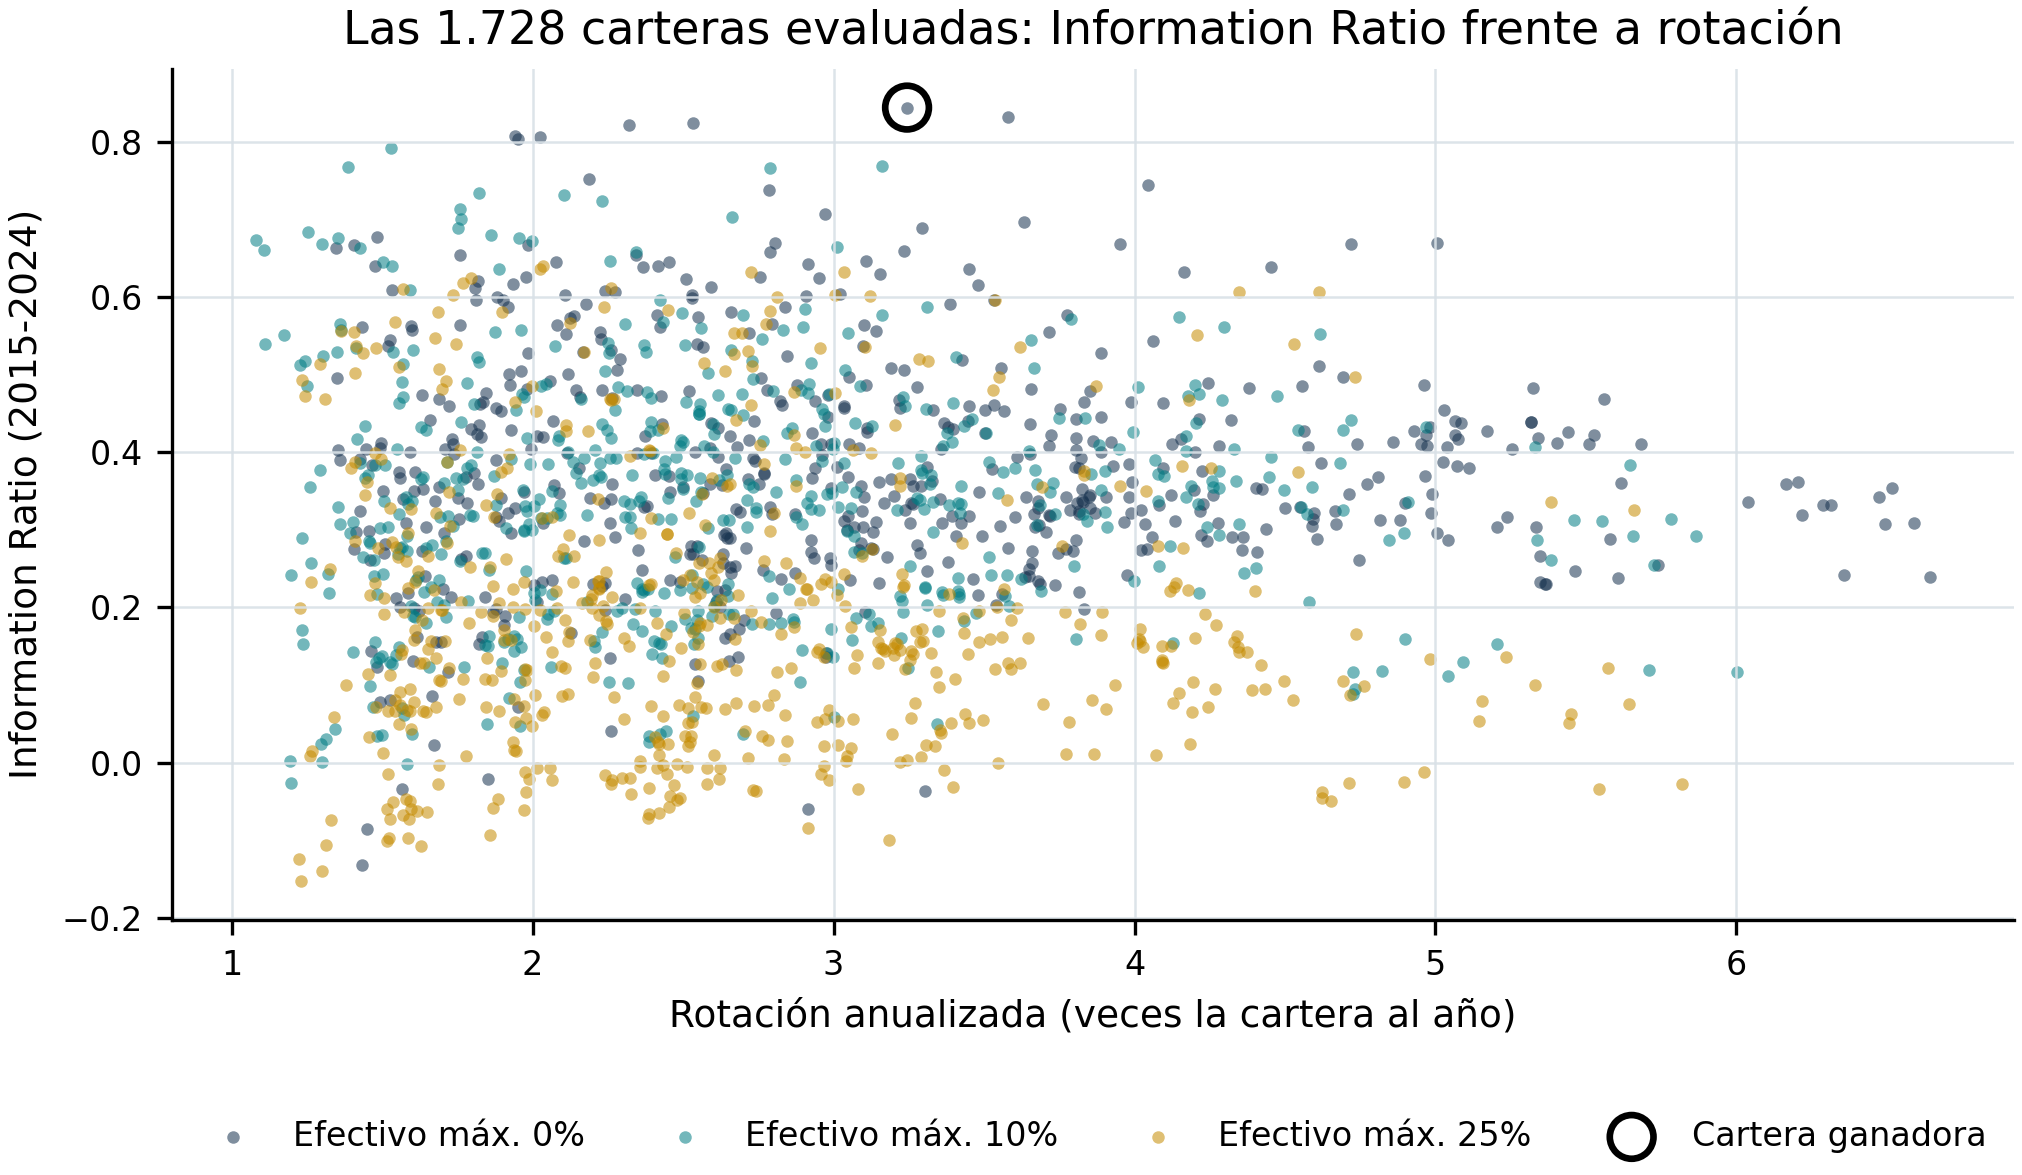
\includegraphics[width=0.94\textwidth]{assets/f08_cartera_rejilla.png}
  \caption{Las carteras evaluadas en el plano rotación--Information Ratio. Cada punto es una cartera
  completa, con las seis coordenadas fijadas a la vez; el color codifica el tope de efectivo y el
  círculo negro señala la ganadora.}
  \label{fig:cartera-rejilla}
\end{figure}

La nube de la Figura~\ref{fig:cartera-rejilla} deja ver de entrada que el Information Ratio no es
una función de la rotación: para casi cualquier nivel de turnover existen carteras buenas y
carteras mediocres, de modo que rotar poco no es en sí mismo una virtud ni rotar mucho un defecto.
Lo que sí separa la nube con claridad es el tope de efectivo, cuya banda superior se agrupa en los
topes bajos.

\begin{figure}[H]
  \centering
  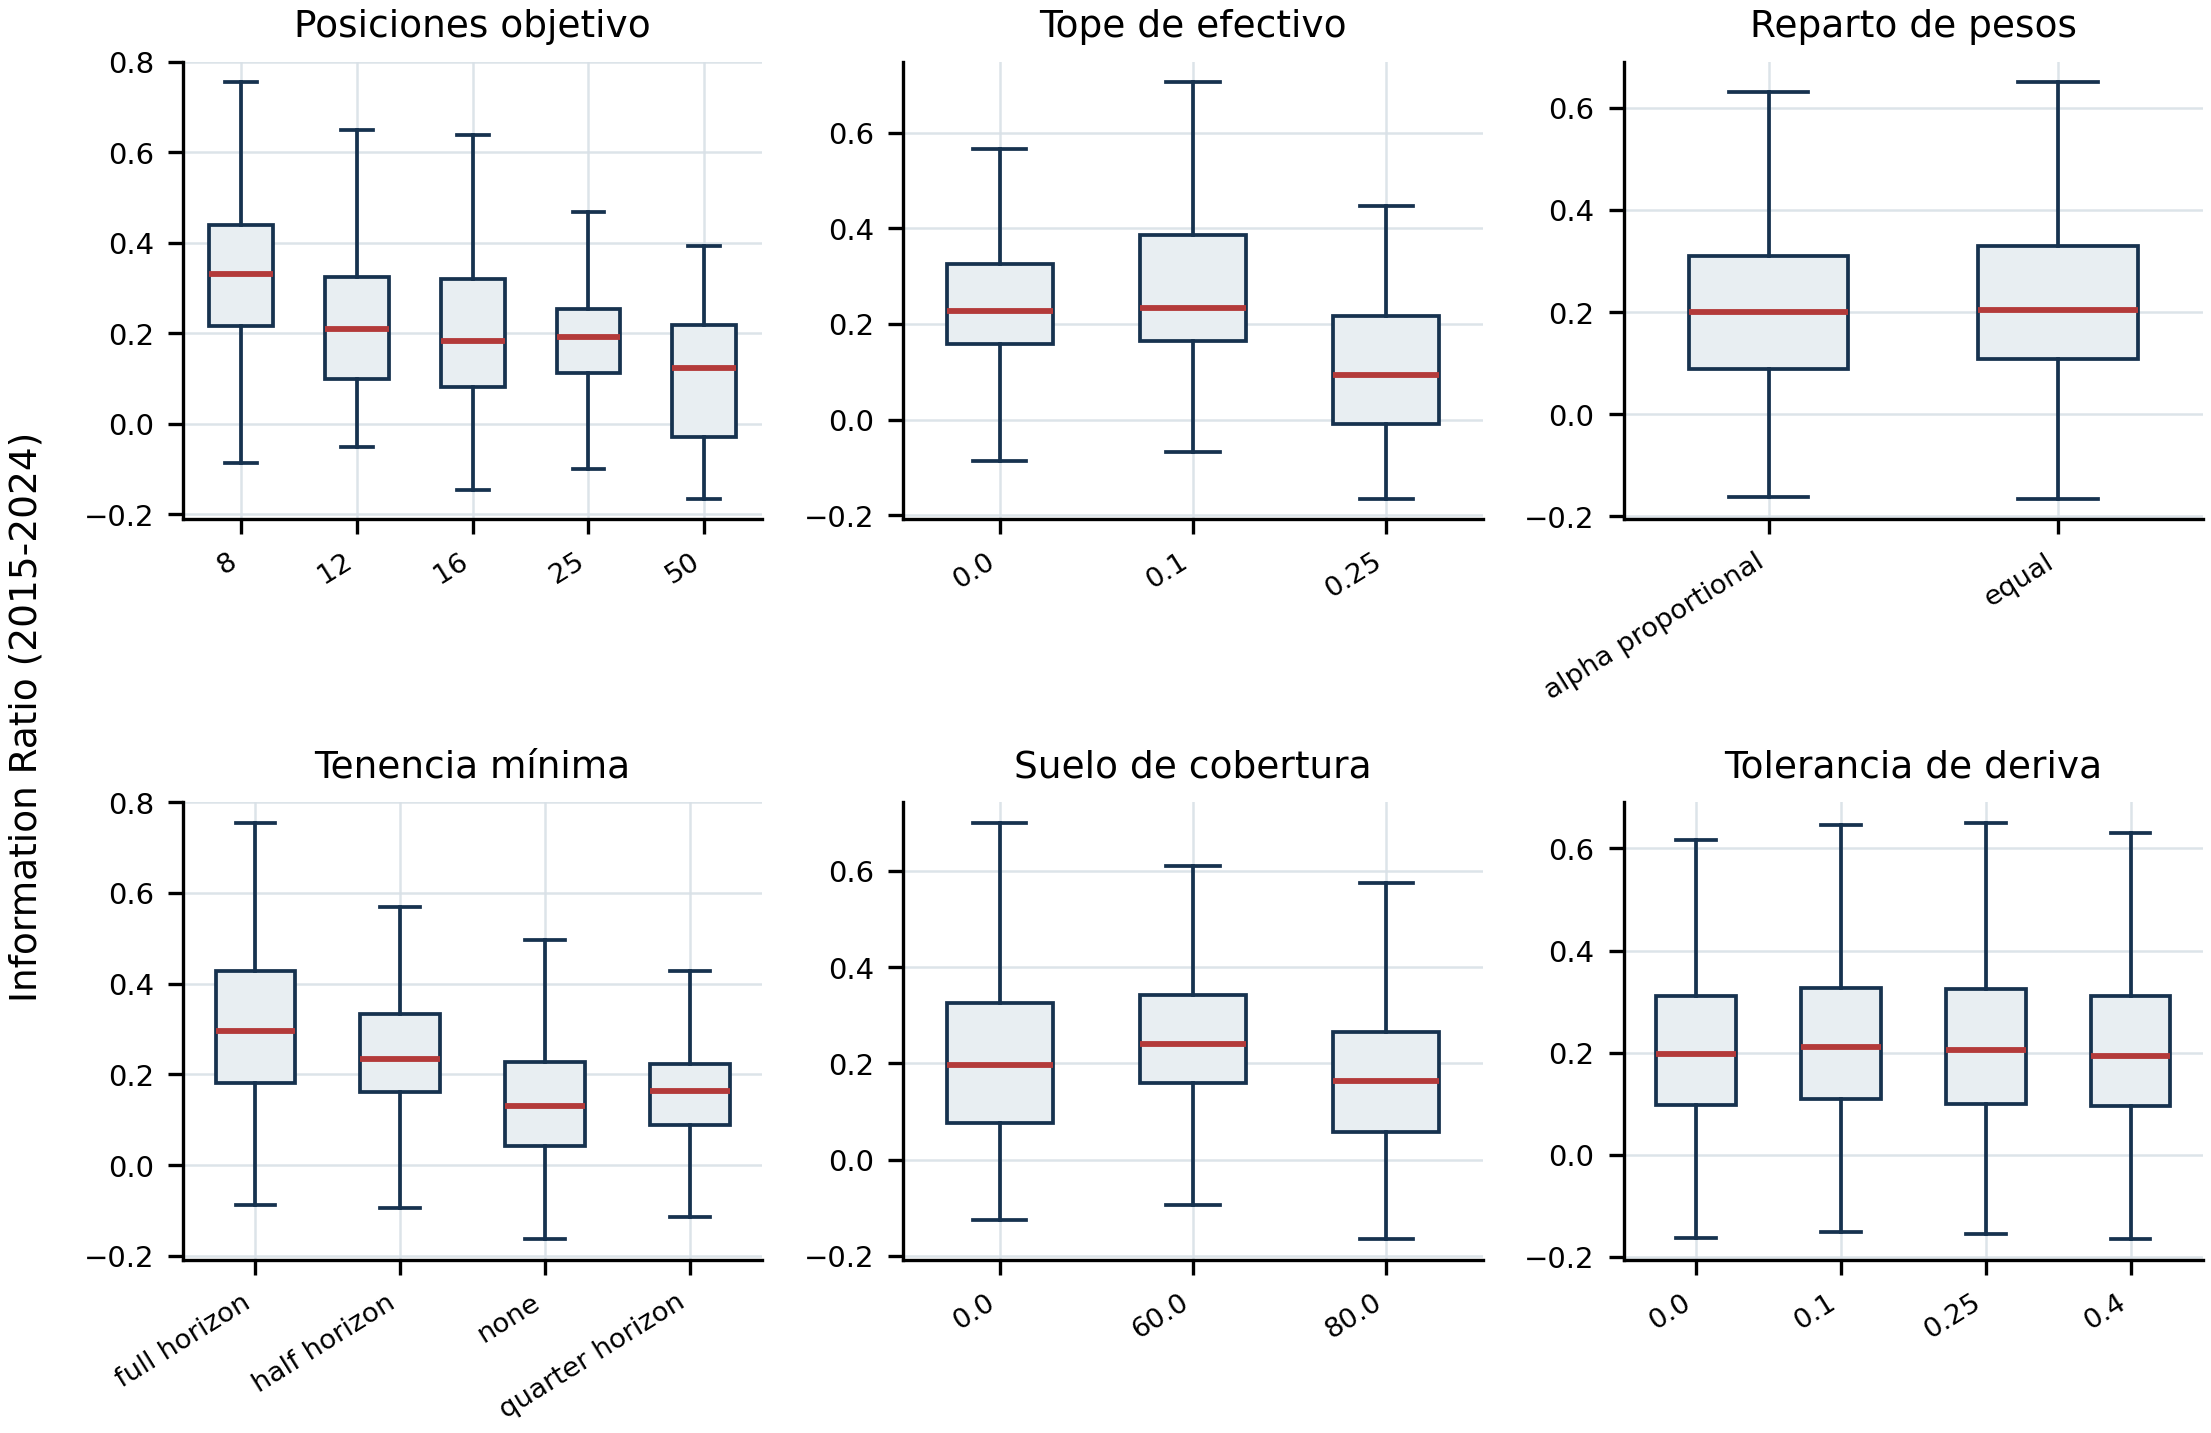
\includegraphics[width=0.96\textwidth]{assets/f08_cartera_marginales.png}
  \caption{Efecto marginal de cada variable sobre el Information Ratio. Cada caja resume todas las
  carteras que comparten ese valor, con las cinco variables restantes variando libremente.}
  \label{fig:cartera-marginales}
\end{figure}

La Figura~\ref{fig:cartera-marginales} traduce a distribuciones lo que la tabla resume en medianas,
y añade una información que la tabla no puede dar: la \emph{forma} del efecto. Las dos variables de
exposición desplazan la distribución del IR de forma inequívoca, mientras que la tolerancia de
deriva apenas la mueve: sus cuatro cajas son casi indistinguibles, lo que significa que esa variable
es, a efectos del Information Ratio, prácticamente inerte. Es una conclusión que el barrido de una
variable cada vez no podía alcanzar, porque no distinguía entre «este valor es mejor» y «esta
variable da igual».

Cada caja resume un \emph{conjunto} de carteras, no una cartera: al fijar una coordenada las otras
cinco siguen variando. Una mediana alta significa que ese valor tiende a funcionar bien acompañado
de casi cualquier cosa, no que baste con adoptarlo. De ahí la aparente contradicción entre las 5
posiciones que maximizan la mediana y las 8 de la ganadora: en el punto concreto donde el tope de
efectivo es cero y el suelo de cobertura es 60, ocho funcionan mejor que cinco, aunque promediando
sobre todos los contextos ocurra lo contrario. Un ascenso por coordenadas habría fijado 5 en el
primer paso y nunca habría vuelto sobre ello.

\section{La cartera ganadora}
\label{sec:cartera-ganadora}


La cartera elegida concentra en ocho posiciones, reparte el peso en proporción al alfa esperado, no
sostiene efectivo, retiene cada posición al menos medio horizonte, corta por debajo del percentil 60
y corrige la deriva al 10\,\%. Conviene precisar en qué se diferencia exactamente de la cartera del
modelo, porque es lo que convierte la comparación en un experimento legible: comparten el número de
posiciones, el reparto de pesos y el suelo de cobertura, y difieren en tres cosas --- renuncia al
efectivo (del 25\,\% al 0\,\%), impone una tenencia mínima de medio horizonte donde antes no había
ninguna, y estrecha la corrección de deriva de 0,25 a 0,1. Es, por tanto, una cartera \emph{menos}
defensiva, no más concentrada. Y eso es coherente con lo que mide el Information Ratio: el efectivo
sin remunerar reduce el numerador de forma sistemática y su ahorro de varianza no lo compensa.

\begin{table}[H]
  \centering
  \small
  \caption{La cartera ganadora frente a la cartera del modelo.}
  \label{tab:cartera-ganadora}
  \begin{tabular}{lrrrr}
\toprule
Métrica & Cartera del modelo & Cartera ganadora & Diferencia & Era reservada \\
\midrule
Information Ratio & 0,339 & 0,844 & 0,505 & 0,304 \\
Exceso geométrico & 2,61\% & 6,97\% & 4,36\% & 2,56\% \\
Rotación anualizada & 3,58 & 3,24 & -0,33 & 3,91 \\
Máxima caída & 26,97\% & 28,40\% & 1,42\% & 12,09\% \\
Años que baten & 70\% & 80\% & 10\% & 50\% \\
\bottomrule
\end{tabular}

  \caption*{Las dos primeras columnas se miden sobre 2015--2024; la última, sobre la era reservada,
  que no intervino en la elección.}
\end{table}

La mejora en la ventana de selección es grande y era esperable, porque es justo la ventana sobre la
que se optimizó: el Information Ratio pasa de 0,339 a 0,844 y el exceso geométrico de 2,61\,\% a
6,97\,\%. Lo que no era esperable, y constituye el resultado central de este trabajo, aparece en la
última columna.

\subsection*{Selección frente a confirmación}

\begin{figure}[H]
  \centering
  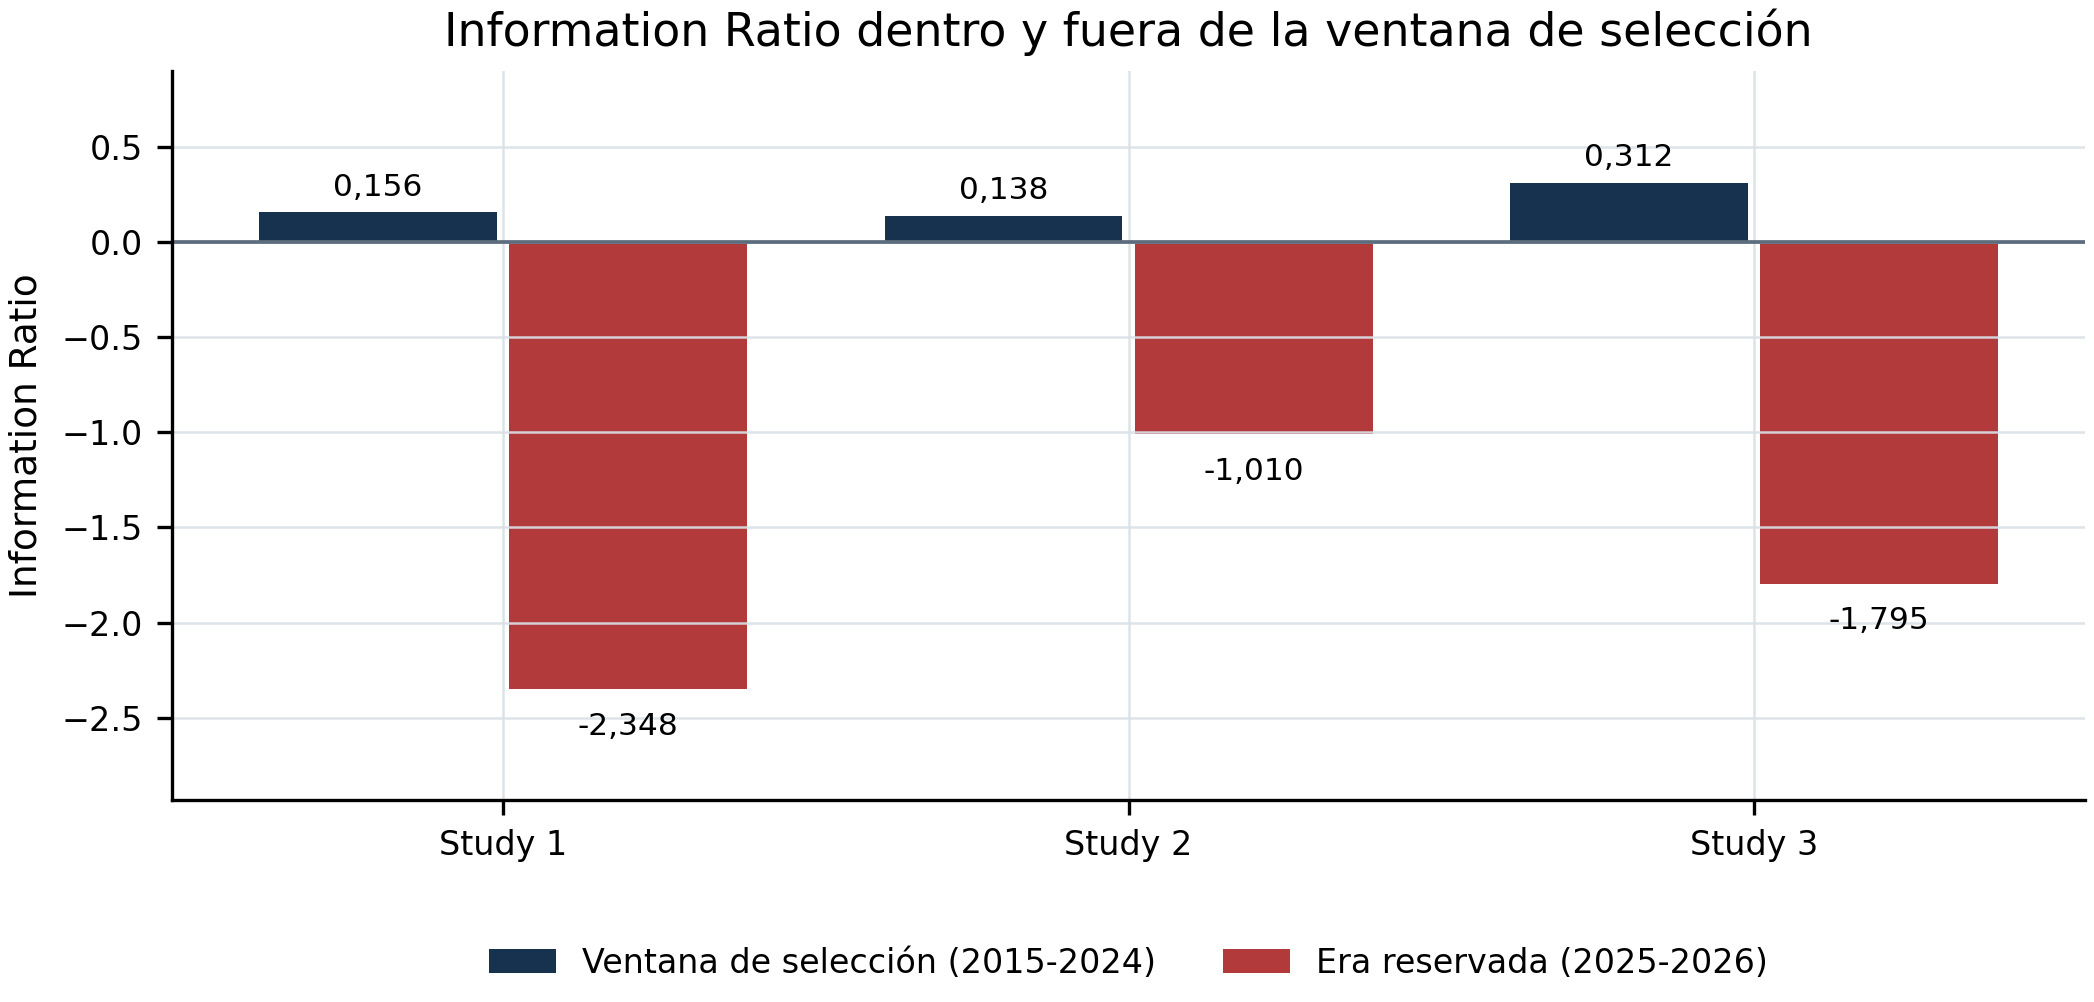
\includegraphics[width=0.92\textwidth]{assets/f09_seleccion_vs_reservada.png}
  \caption{Information Ratio dentro y fuera de la ventana de selección, pasada a pasada de la
  cadena, con la cartera por defecto del catálogo.}
  \label{fig:seleccion-vs-reservada}
\end{figure}

La Figura~\ref{fig:seleccion-vs-reservada} documenta el problema que la optimización de cartera
vino a resolver, y conviene leerla antes que la solución. Las tres pasadas de la cadena mejoran
monótonamente dentro de la ventana de selección --- 0,189, 0,294 y 0,339 de Information Ratio --- y
\emph{se degradan} monótonamente fuera de ella: 0,898, 0,476 y $-1{,}167$. Con la cartera por
defecto, la tercera pasada, que es la mejor de la cadena en selección, es la peor con diferencia en
la era reservada, donde pierde un 11,29\,\% frente al índice sin batirlo ni un solo año. Es la firma
clásica del sobreajuste por búsqueda: cada pasada aprendía algo más sobre la ventana con la que se
decidía y algo menos sobre el mundo.

El hallazgo es que esa degradación \textbf{no procedía del modelo}. Con la cartera optimizada, la
misma señal, sin reentrenar nada y sin tocar una sola variable predictiva, obtiene en la era
reservada un exceso de $+2{,}56$\,\% y un Information Ratio de $+0{,}304$, batiendo al índice en la
mitad de los años en lugar de en ninguno. La ordenación transversal siempre había sido válida fuera
de muestra --- su Rank-IC en esa era es $+0{,}0441$, positivo aunque menor que en selección ---; lo
que fallaba era la maquinaria que la convertía en posiciones.

Este resultado exige dos cautelas explícitas y el trabajo no las oculta. La primera es de tamaño
muestral: la era reservada abarca seis cohortes y 1,41 años de cartera, de modo que
«bate en la mitad de los años» significa uno de dos, y ningún contraste construido sobre esa
cantidad de datos puede ser concluyente. La segunda es de multiplicidad: la cartera ganadora es la
mejor de 1.728, y aunque ninguna de ellas pudo ver la era reservada durante la selección, el hecho
de que la ganadora generalice no queda demostrado por un único periodo de confirmación. Lo que sí
puede afirmarse, y es lo que se afirma, es que la hipótesis «la señal no se traslada a rentabilidad
fuera de muestra» queda desmentida en las condiciones medidas, y que la gestión de cartera --- no la
capacidad predictiva --- era el cuello de botella.

\section{Resultados económicos completos}
\label{sec:economia-completa}

Con la cartera ya elegida, la evaluación sobre la serie completa produce las cifras que este
apartado desarrolla. Entre 2015 y 2024 la cartera obtiene CAGR 21,06\,\% frente a 13,17\,\% de SPY;
el exceso geométrico es 6,97\,\%, el IR 0,844, el máximo drawdown 28,40\,\% y el benchmark se bate
en 8 de 10 años. El coste acumulado, 4,74\,\%, y el turnover anualizado, 324,43\,\%, son centrales
para interpretar el resultado: la implementación captura sólo una parte de la señal disponible, y lo
hace pagando fricción por el camino.

\begin{table}[H]
  \centering
  \small
  \caption{Las tres ventanas de evaluación, con su papel declarado.}
  \label{tab:tres-ventanas}
  \begin{tabular}{lrrr}
\toprule
Métrica & Selección 2015–2024 & Confirmación 2025–2026 & Curva completa \\
\midrule
CAGR de cartera & 21,06\% & 22,23\% & 21,04\% \\
CAGR de SPY & 13,17\% & 19,18\% & 13,81\% \\
Exceso geométrico & 6,97\% & 2,56\% & 6,35\% \\
Information ratio & 0,844 & 0,304 & 0,753 \\
Máximo drawdown & 28,40\% & 12,09\% & 28,40\% \\
Años por encima de SPY & 80,00\% & 50,00\% & 75,00\% \\
Alfa anual media & 7,17\% & 1,91\% & 6,29\% \\
Peor alfa anual & -8,30\% & -2,73\% & -8,30\% \\
Turnover anualizado & 324,43\% & 391,35\% & 333,35\% \\
Efectivo medio & 0,00\% & 0,00\% & 0,00\% \\
Coste acumulado & 4,74\% & 0,88\% & 5,63\% \\
Periodos & 117 & 18 & 135 \\
\bottomrule
\end{tabular}

  \caption*{Cifras de la cartera adoptada, no de la que el catálogo recomienda. Selección: se
  tomaron decisiones sobre ella. Confirmación: reservada, ninguna decisión la utilizó. Curva
  completa: descriptiva, no probatoria.}
\end{table}

Dos observaciones sobre la tabla condicionan su lectura. La primera es que el efectivo medio es
\textbf{cero en las tres ventanas}: la cartera ganadora renuncia por completo a la liquidez, de modo
que su resultado no puede atribuirse a haber estado fuera del mercado en los momentos oportunos.
Está siempre invertida, y su exceso procede íntegramente de qué acciones eligió.

La segunda es que el turnover \emph{sube} en la era reservada, de 324\,\% a 391\,\%, mientras el
coste acumulado se mantiene bajo por lo corto del periodo. No hay aquí un cambio de comportamiento
del sistema: con una cartera de ocho posiciones y sin colchón de efectivo, cada cambio de opinión de
la señal obliga a una rotación completa de la plaza afectada.

\begin{figure}[H]
  \centering
  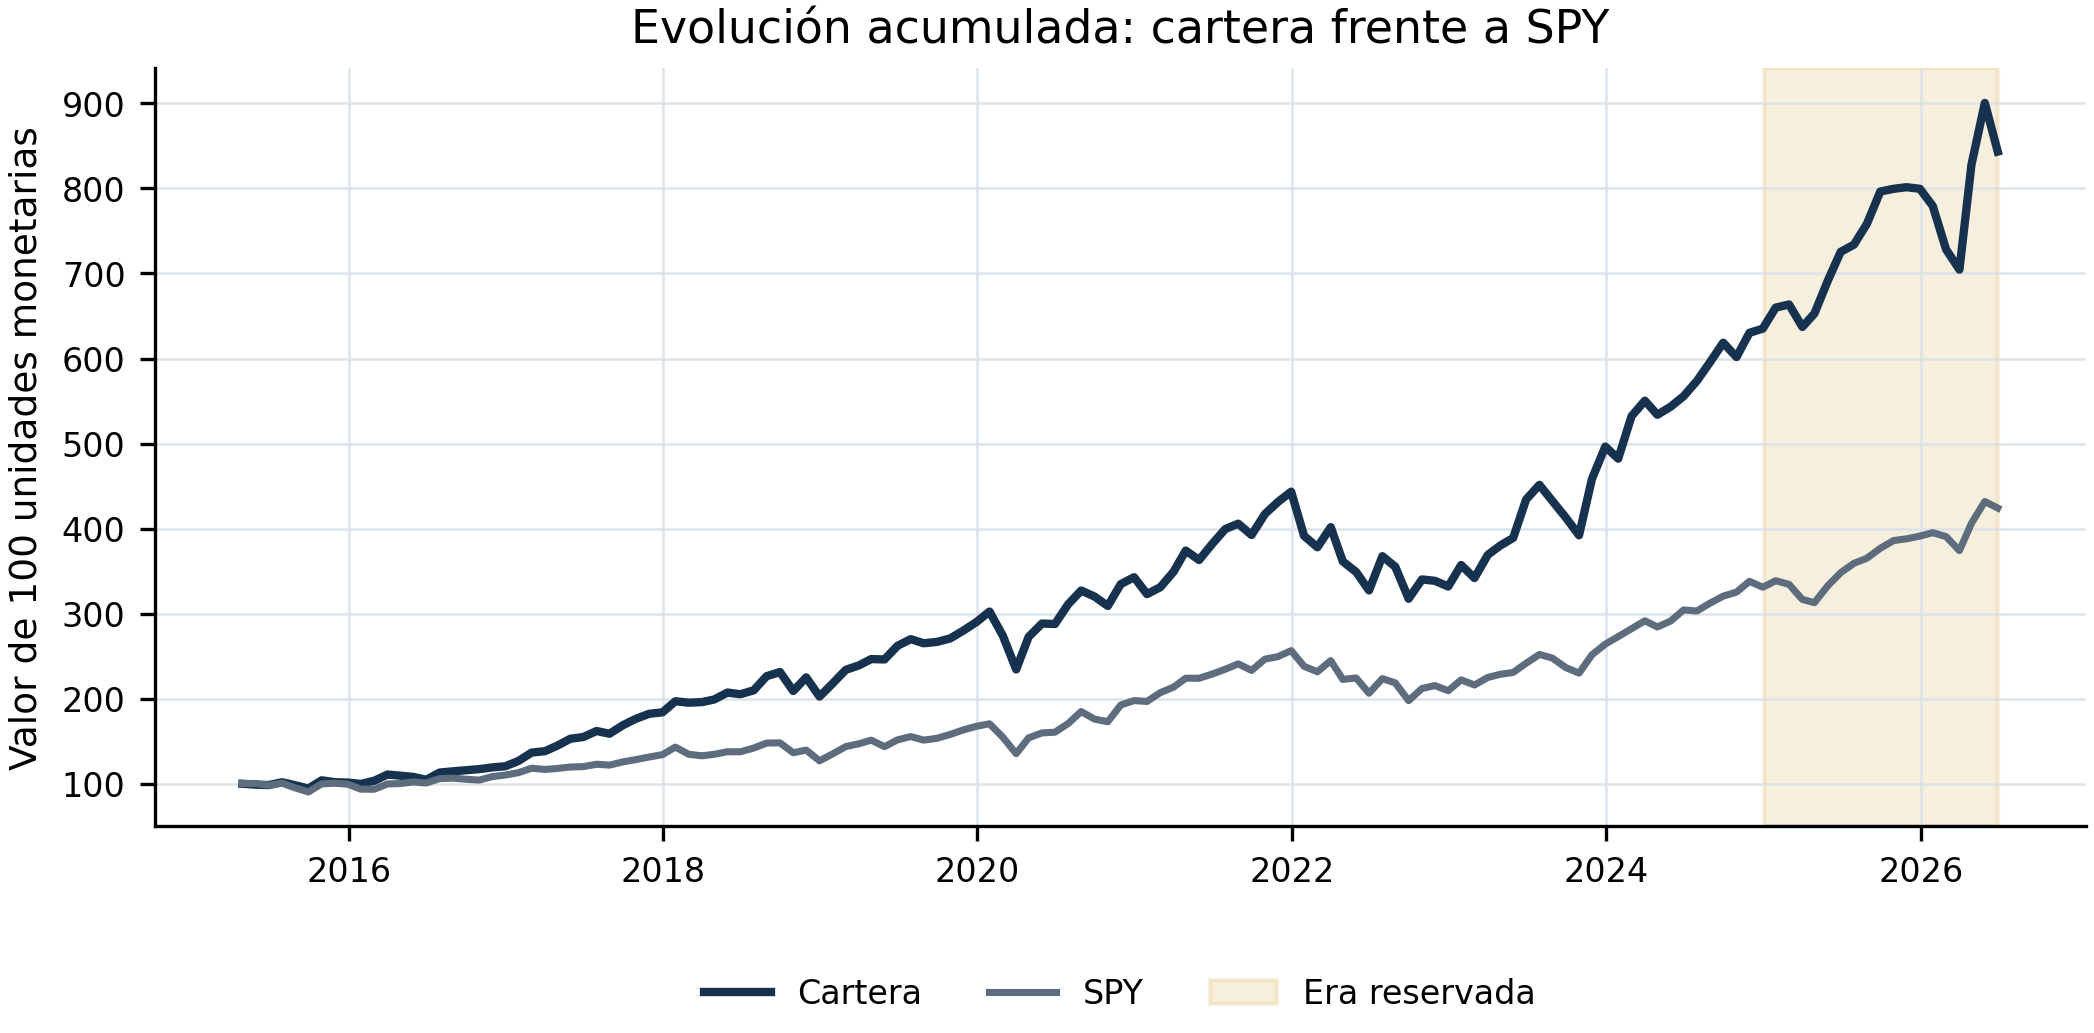
\includegraphics[width=0.96\textwidth]{assets/f07_equity.png}
  \caption{Curva de patrimonio de la cartera ganadora y SPY. La región dorada es confirmación
  reservada, no selección.}
  \label{fig:equity}
\end{figure}

La curva de la Figura~\ref{fig:equity} permite una lectura que las medias agregadas no dan: la
ventaja no se construye en un salto sino de forma acumulativa, y el tramo dorado --- la era
reservada --- no rompe la trayectoria. La Figura~\ref{fig:drawdown} muestra el reverso de esa misma
serie.

\begin{figure}[H]
  \centering
  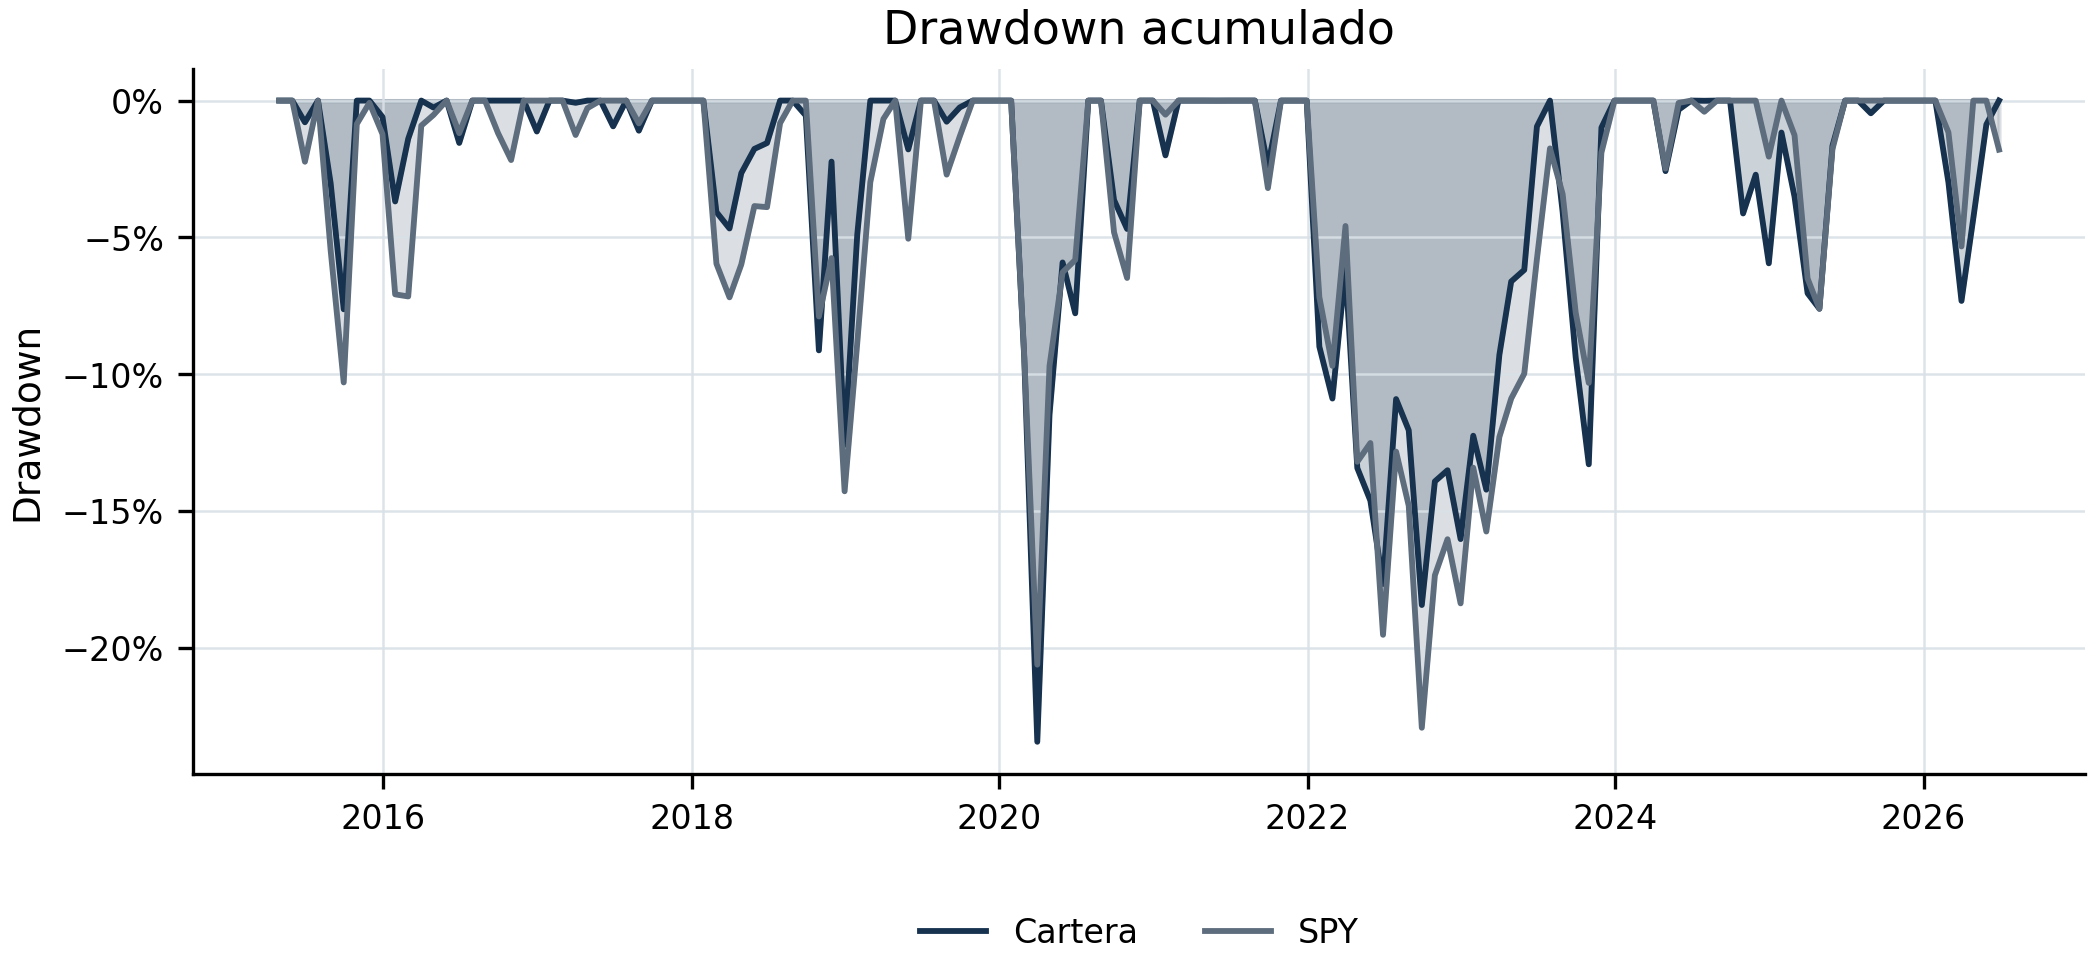
\includegraphics[width=0.92\textwidth]{assets/f07_drawdown.png}
  \caption{Drawdown acumulado de la cartera ganadora y SPY.}
  \label{fig:drawdown}
\end{figure}

El drawdown máximo de 28,40\,\% es la contrapartida de haber renunciado al efectivo: 1,42 puntos más
que la cartera del modelo, que mantenía un colchón del 25\,\%. La optimización no redujo el riesgo
de caída, lo aceptó a cambio de numerador. Que el drawdown de una cartera de ocho nombres sea
comparable al de un índice de quinientos es un resultado favorable, pero no debe leerse como control
de riesgo: es consecuencia de la señal, no de una política de exposición, que el sistema no tiene.


\begin{table}[H]
  \centering
  \scriptsize
  \caption{Resultado anual de la cartera ganadora.}
  \label{tab:anual}
  \begin{tabular}{lrrrrrrr}
\toprule
Año & Cartera & SPY & Alfa & MDD & IR & Efectivo & Turnover \\
\midrule
2015 & 1,27\% & -0,63\% & 1,91\% & 7,30\% & 0,434 & 0,00\% & 158,59\% \\
2016 & 19,00\% & 10,88\% & 7,32\% & 5,59\% & 0,814 & 0,00\% & 379,81\% \\
2017 & 52,56\% & 21,71\% & 25,35\% & 1,98\% & 3,877 & 0,00\% & 308,32\% \\
2018 & 10,10\% & -5,40\% & 16,38\% & 12,50\% & 1,887 & 0,00\% & 291,11\% \\
2019 & 43,38\% & 32,05\% & 8,57\% & 1,80\% & 1,553 & 0,00\% & 332,78\% \\
2020 & 18,13\% & 18,02\% & 0,09\% & 22,52\% & 0,067 & 0,00\% & 361,61\% \\
2021 & 29,34\% & 29,71\% & -0,29\% & 3,28\% & 0,032 & 0,00\% & 265,83\% \\
2022 & -25,16\% & -18,38\% & -8,30\% & 20,96\% & -0,928 & 0,00\% & 120,14\% \\
2023 & 49,61\% & 26,18\% & 18,57\% & 13,14\% & 1,679 & 0,00\% & 468,60\% \\
2024 & 27,94\% & 25,34\% & 2,07\% & 3,01\% & 0,213 & 0,00\% & 476,39\% \\
2025 & 25,90\% & 18,17\% & 6,55\% & 3,99\% & 1,056 & 0,00\% & 330,53\% \\
2026 & 5,48\% & 8,43\% & -2,73\% & 9,60\% & -0,123 & 0,00\% & 256,49\% \\
\bottomrule
\end{tabular}

  \caption*{Turnover anualizado; efectivo medio.}
\end{table}

El detalle anual desmiente que el exceso agregado proceda de un año excepcional. La cartera bate al
índice en ocho de los diez años de la ventana de selección, con un alfa medio de 7,17\,\% y una
mediana de 4,70\,\%: la distribución está desplazada, no arrastrada por una cola. Los dos años
negativos se analizan más adelante, junto con la era reservada.

\section{Órdenes, rotación y costes}
\label{sec:rotacion}

Un turnover del 324\,\% anualizado exige explicación. La Tabla~\ref{tab:ordenes} lo descompone por
motivo declarado de cada orden.

\begin{table}[H]
  \centering
  \small
  \caption{Descomposición del flujo de cartera por motivo de orden.}
  \label{tab:ordenes}
  \begin{tabular}{lrrr}
\toprule
Motivo de la orden & Órdenes & \% del flujo & Coste \\
\midrule
net\_edge\_over\_worst & 40 & 36,5\% & 3,43 \\
displaced\_by\_net\_edge & 40 & 35,0\% & 3,31 \\
rebalance & 61 & 17,6\% & 2,18 \\
initial\_fill & 8 & 7,3\% & 0,30 \\
cash\_floor\_fill & 2 & 1,8\% & 0,25 \\
missing\_current\_score & 2 & 1,8\% & 0,24 \\
\textbf{Total} & \textbf{153} & \textbf{100,0\%} & \textbf{9,70} \\
\bottomrule
\end{tabular}

  \caption*{El flujo es la suma de $|\Delta w|$ de cada orden. El coste agrega comisión y
  \textit{slippage} efectivamente cargados.}
\end{table}


El desglose revela que la rotación tiene \textbf{dos fuentes de tamaño comparable, y de naturaleza
muy distinta}. La primera es el cambio de opinión de la señal:
\texttt{net\_edge\_over\_worst} y \texttt{displaced\_by\_net\_edge}, que son las dos caras de una
misma operación, suman el 37,0\,\% del flujo. La segunda es el \texttt{rebalance}, con un
38,2\,\%, que no cambia \emph{qué} se tiene sino sólo el peso de lo que ya se tiene. El resto ---
compras iniciales 10,9\,\%, ventas por caer bajo el suelo de cobertura 9,0\,\% y dos motivos
residuales --- completa el cuadro.

Las dos fuentes se distinguen además por su granularidad. El \texttt{rebalance} son 408 órdenes
pequeñas, mientras que la rotación por ventaja neta son 104 órdenes unas cuatro veces mayores cada
una. Y ambas cuestan lo suyo: el \texttt{rebalance} se lleva 8,08 de los 21,19 puntos de coste
acumulado, prácticamente lo mismo que la rotación.

Cada fuente responde a una palanca distinta, y sólo una está disponible. La rotación por ventaja
neta es estructural: el sistema \emph{re-decide todos los meses} sobre una señal cuyo horizonte es
de \emph{doce}, de modo que cada snapshot vuelve a comparar las posiciones con todo el universo y
basta una diferencia neta que supere el umbral para que se ejecute un intercambio que la señal, a
doce meses vista, quizá no habría pedido. Su palanca es \artefacto{snapshot\_step\_months}, pero es
una variable \emph{predictiva}: cambiarla obligaría a rehacer la selección secuencial completa, y de
hecho fue la primera decisión del estudio, donde la cadencia mensual ganó con una ventaja pareada de
$+0{,}0208$ frente a la trimestral. Queda así un conflicto real entre dos objetivos legítimos ---
más cohortes para decidir mejor frente a menos rotación para implementar mejor --- que este trabajo
documenta pero no resuelve.

El \texttt{rebalance}, en cambio, depende de \artefacto{rebalance\_drift\_tolerance}, que sí es una
variable de cartera y sí se optimizó. La rejilla eligió 0,1 sobre una escala que llega a 0,4, es
decir, una corrección de deriva estrecha. Y aquí aparece un dato que conviene no pasar por alto:
esa misma variable es, según la Tabla~\ref{tab:cartera-influencia}, la penúltima en capacidad de
mover el Information Ratio (0,016). El sistema está pagando con ella su mayor partida de flujo de
órdenes a cambio de una diferencia marginal en el criterio que se optimizó. No es un defecto del
procedimiento --- 0,1 medía mejor que las alternativas, y por poco que sea la rejilla lo prefirió
---, pero sí señala dónde habría margen para reducir fricción casi sin coste en Information Ratio.

\subsection*{Rotación, coste y exceso año a año}

La Tabla~\ref{tab:anual} permite comprobar que ese turnover no compra rentabilidad. No hay relación
monótona entre rotar más y obtener más exceso: el peor año de la ventana, 2022, tuvo la rotación más
baja de toda la serie, de modo que su pérdida frente al índice no se explica por fricción sino por
composición. El coste acumulado de 4,74 puntos porcentuales frente a un exceso geométrico de
6,97\,\% no es despreciable --- antes de costes la ventaja sería sustancialmente mayor ---, pero es
un peaje que la cartera paga para expresar la señal, no la fuente de su resultado.

Conviene subrayar un dato de la optimización que apunta en la misma dirección: la cartera ganadora
rota \emph{menos} que la del catálogo (3,24 frente a 3,58 veces al año) y aun así obtiene mucho más
exceso. La mejora no se compró rotando más. Es coherente con lo que muestra la
Figura~\ref{fig:cartera-rejilla}: en la nube de las 1.728 carteras, el Information Ratio y el
turnover no guardan relación clara, y las mejores combinaciones aparecen repartidas por todo el
rango de rotación.

\subsection*{Cuánta señal llega a materializarse}
\label{sec:transferencia}

La ley fundamental de la gestión activa, introducida en el Capítulo~\ref{chap:estado-arte},
descompone el resultado de una cartera en calidad de señal, amplitud y coeficiente de transferencia.
Este trabajo no dispone de ese coeficiente para la cartera adoptada --- el Portfolio Study no
recalcula la atribución sobre su ganadora ---, pero sí tiene dos observaciones que sostienen el
mismo argumento sin necesidad de esa cifra.

La primera es que en la cadena de Model Studies la transferencia creció de forma sostenida (0,178,
0,234 y 0,328): cada pasada no sólo ordenaba algo mejor, sino que además llevaba a la cartera una
fracción mayor de lo que ordenaba. Eso identificó la implementación como la palanca disponible y
motivó el Portfolio Study. La segunda es que el salto de Information Ratio de 0,339 a 0,844
\textbf{sobre la misma señal congelada} mide exactamente esa magnitud por otra vía: como el
numerador predictivo no cambió, todo el incremento procede de que la cartera desperdicia menos.

\section{Los ocho perfiles de inversor}
\label{sec:perfiles}

Hasta aquí la cartera ha comprado siempre las mejores acciones según el meta-agente. Un inversor
real rara vez opera así: tiene un estilo, y ese estilo le hace preferir unas empresas sobre otras
\emph{dentro} de las que su sistema considera buenas. Los ocho perfiles formalizan esa idea y
responden a una pregunta concreta: ¿habría mejorado el resultado alguien que, teniendo esta misma
señal y esta misma gestión, la hubiera filtrado según su criterio?

\subsection*{Qué es exactamente un perfil}

Un perfil no es un modelo distinto ni una cartera distinta: es una \textbf{reordenación de la señal
ya congelada}, y opera en dos pasos.

Primero acota el universo. Sólo son elegibles las acciones que el meta-agente sitúa por encima del
percentil 60, de modo que ningún perfil puede comprar algo que el sistema considere malo: todos
eligen dentro del mismo conjunto de candidatas.

Después reordena ese conjunto combinando los rangos de los cinco agentes con pesos fijos, declarados
de antemano. El resultado sustituye al \texttt{meta\_rank} y la cartera lo consume igual que antes.
Los pesos pueden ser \emph{negativos} cuando el estilo apuesta en contra de un agente --- es el caso
del \texttt{contrarian} frente al momentum ---, y conviene tener presente una convención del
catálogo: en \texttt{risk} el rango alto significa \emph{menos} riesgo, de modo que un peso positivo
prioriza baja volatilidad y uno negativo la tolera.

\begin{table}[H]
  \centering
  \footnotesize
  \caption{Los ocho perfiles: qué hipótesis de estilo representa cada uno.}
  \label{tab:perfiles-def}
  % Definición de los ocho perfiles: transcrita de PROFILE_WEIGHTS en
% module/evaluation/profiles.py. No es un artefacto del estudio sino la
% configuración del código, por eso se escribe a mano y no se genera.
\begin{tabularx}{\textwidth}{lXl}
\toprule
Perfil & Hipótesis de estilo & Pesos sobre los rangos de agente \\
\midrule
\texttt{balanced} &
El meta-agente sin alterar. Es la referencia: mide qué ocurre cuando \emph{no} se impone estilo &
\texttt{meta} 1,00 \\
\addlinespace
\texttt{defensive} &
Preservación de capital: baja volatilidad y negocios sólidos &
\texttt{risk} 0,60 · \texttt{qual} 0,35 · \texttt{val} 0,05 \\
\addlinespace
\texttt{quality} &
\textit{Compounder} tipo Buffett: negocios excelentes y duraderos &
\texttt{qual} 0,70 · \texttt{grow} 0,20 · \texttt{val} 0,10 \\
\addlinespace
\texttt{growth} &
Crecimiento como motor, pero de calidad; el momentum confirma la tendencia &
\texttt{grow} 0,60 · \texttt{qual} 0,25 · \texttt{mom} 0,15 \\
\addlinespace
\texttt{value} &
Empresas infravaloradas; calidad y riesgo filtran las \textit{value traps} &
\texttt{val} 0,70 · \texttt{qual} 0,15 · \texttt{risk} 0,15 \\
\addlinespace
\texttt{garp} &
\textit{Growth at a reasonable price}: crecer con disciplina de precio &
\texttt{grow} 0,40 · \texttt{val} 0,35 · \texttt{qual} 0,25 \\
\addlinespace
\texttt{contrarian} &
Comprar lo castigado: apuesta \emph{en contra} del momentum reciente &
\texttt{mom} $-0{,}55$ · \texttt{val} 0,30 · \texttt{risk} 0,15 \\
\addlinespace
\texttt{momentum} &
Fuerza de precio pura, aceptando la volatilidad que la acompaña &
\texttt{mom} 0,75 · \texttt{risk} $-0{,}25$ \\
\bottomrule
\end{tabularx}

\end{table}

Como la reordenación cambia qué acciones se compran, el alfa esperado deja de corresponder al orden
vigente. Por eso la calibración de percentil a rentabilidad \textbf{se recalcula sobre el ranking
nuevo}: si no se hiciera, el perfil operaría con expectativas referidas a un orden que ya no usa, y
sus umbrales en puntos básicos decidirían sobre posiciones ajenas.

\subsection*{Qué le pasó a cada estilo}

\begin{table}[H]
  \centering
  \small
  \caption{Los ocho perfiles de inversor evaluados con la cartera ganadora.}
  \label{tab:perfiles-cartera}
  \begin{tabular}{lrrrrrr}
\toprule
Perfil & IR sel. & Exceso sel. & Turnover & Efectivo & IR reserv. & Exceso reserv. \\
\midrule
balanced & 0,844 & 6,97\% & 3,24 & 0,00\% & 0,304 & 2,56\% \\
defensive & 0,570 & 3,73\% & 2,51 & 0,00\% & -0,607 & -5,70\% \\
quality & 0,312 & 2,06\% & 3,40 & 0,00\% & -0,635 & -9,09\% \\
growth & 0,212 & 1,04\% & 3,93 & 0,00\% & 0,318 & 4,14\% \\
value & 0,190 & 1,16\% & 3,82 & 0,00\% & -0,513 & -4,94\% \\
garp & 0,112 & 0,51\% & 3,89 & 0,00\% & -0,779 & -8,76\% \\
contrarian & 0,057 & -0,40\% & 4,33 & 0,00\% & 0,414 & 4,44\% \\
momentum & 0,017 & -0,77\% & 5,98 & 0,00\% & 1,889 & 41,59\% \\
\bottomrule
\end{tabular}

\end{table}

El resultado principal es que \textbf{ninguno de los siete estilos mejora a la señal sin reordenar}.
El perfil \texttt{balanced} domina la ventana de selección con un Information Ratio de 0,844 frente
al 0,570 del siguiente, y dos estilos llegan a exceso negativo. La ordenación aprendida ya contiene,
por tanto, lo que los perfiles intentan imponer desde fuera.

Lo interesante es que el orden entre ellos \emph{no es arbitrario}: se predice casi por completo
desde la calidad de los agentes que cada uno pondera, medida en la Tabla~\ref{tab:agentes}. El mejor
de los siete es \texttt{defensive} (IR 0,570), que carga el 60\,\% en \texttt{risk}, el agente de
mayor Rank-IC (0,1227). El peor es \texttt{momentum} (IR 0,017), que carga el 75\,\% en el agente de
Rank-IC 0,0005 --- indistinguible de cero --- y además penaliza a \texttt{risk}. Entre medias,
\texttt{quality}, \texttt{growth}, \texttt{value} y \texttt{garp} se reparten pesos entre agentes
cuyo Rank-IC ronda 0,01--0,02, y sus IR quedan agrupados entre 0,112 y 0,312.

La lectura es coherente con todo el capítulo anterior: un perfil no añade información, sólo cambia
el peso relativo de la que ya existe. Cuando ese cambio desplaza el peso hacia un agente peor, el
resultado empeora en proporción. El caso de \texttt{contrarian} lo confirma desde el otro extremo:
con peso \emph{negativo} sobre el agente más débil obtiene 0,057, mejor que apostar a favor de él
pero aún muy por debajo de no reordenar nada.

Hay además un coste operativo que la tabla hace visible. Los estilos más agresivos rotan más sin
obtener más exceso: \texttt{momentum} alcanza un turnover de 5,98 veces al año --- casi el doble que
el 3,24 de \texttt{balanced} --- para terminar con exceso negativo. La reordenación no sólo no
aporta señal: cuesta fricción.

La era reservada, en cambio, invierte el orden casi por completo, y el dato merece reportarse
precisamente porque incomoda: \texttt{momentum}, el peor perfil de la ventana de selección con un
Information Ratio de 0,017, es el mejor con diferencia en 2025--2026, con 1,889 y un exceso del
41,59\,\%. La tentación de leer ahí un hallazgo debe resistirse. Seis cohortes no permiten ordenar
ocho estilos de inversión, y un periodo tan corto está dominado por qué régimen de mercado le tocó
en suerte a cada sesgo. Lo que la comparación sí sugiere, y de forma consistente con el resto del
capítulo, es que el orden entre perfiles no es una propiedad estable de la señal sino del régimen, y
que por eso mismo el protocolo hace bien en no elegir perfil por su rentabilidad.

\section{Años adversos y significado de la era reservada}
\label{sec:era-reservada}

Los años con alfa negativo de la ventana de selección, 2021 y 2022, son informativos. En 2021 la
cartera quedó a 0,29 puntos porcentuales del índice, una diferencia que no requiere explicación
estructural. En 2022, en cambio, perdió 8,30 puntos en un año de caída generalizada, y lo hizo con
la rotación más baja de toda la serie (1,20): no fue un problema de fricción sino de composición,
lo que resulta coherente con un sistema que ordena por atractivo relativo y no gestiona la
exposición direccional al mercado.

Es una limitación real de diseño, y conviene enunciarla como tal: el sistema decide \emph{qué}
comprar, no \emph{cuánto} estar expuesto. La política de efectivo es lo más parecido a una palanca
de exposición que tiene, y la cartera ganadora la fija en cero. El resultado es una cartera que
participa íntegramente de las caídas del mercado y aspira a superarlas en términos relativos, no a
evitarlas.

La era reservada ofrece el contraste decisivo del trabajo, y su lectura depende por completo de qué
cartera se use para materializar la señal. Con la cartera optimizada, el CAGR es 22,23\,\% frente a
19,18\,\% de SPY, el exceso geométrico 2,56\,\%, el IR 0,304 y se bate al índice en uno de los dos
años, con un turnover anualizado de 391,35\,\%. Con la cartera por defecto, la misma señal daba
$-11{,}29$\,\% e IR $-1{,}167$, sin batir al índice ningún año. El Rank-IC de la era, $+0{,}0441$
sobre seis cohortes con el 66,67\,\% de ellas positivas, es idéntico en ambos casos porque no
depende de la cartera: es la señal, y la señal se sostuvo, aunque más débil que el 0,1090 de la
ventana de selección.

Debe informarse junto a su debilidad estadística, que es considerable: sólo seis cohortes tienen
etiqueta cerrada, varias observaciones futuras no han madurado y el número de observaciones
independientes efectivas es aproximadamente uno. El trabajo no convierte esa combinación en una
demostración. Lo que afirma es más modesto y más defendible: en la única ventana que no participó en
ninguna decisión, la ordenación aprendida siguió siendo positiva, y su traducción a rentabilidad
dependió de la construcción de cartera hasta el punto de cambiar de signo.

\subsection*{Qué se sigue de todo esto para el diseño de cartera}

Este capítulo empezó preguntando si una cartera real puede expresar la ordenación aprendida sin
destruirla por el camino. La respuesta es que depende de la cartera, y que la diferencia no es de
grado sino de signo: la rejilla evaluó las seis reglas que gobiernan esa traducción sin reabrir la
selección predictiva, y encontró una configuración que multiplica por 2,5 el Information Ratio de la
ventana de selección y cambia el signo del resultado en la era reservada.

La implicación excede al caso concreto. En este sistema, la construcción de cartera no era un
detalle de implementación sino la variable que decidía si la señal servía para algo, de lo que se
sigue una exigencia metodológica: \textbf{ninguna conclusión sobre la utilidad práctica de un
sistema predictivo es interpretable sin declarar con qué cartera se midió}. Un trabajo que reportase
únicamente el resultado de su cartera por defecto habría concluido que la señal no se traslada fuera
de muestra, y se habría equivocado.

Con esto se cierra la evidencia. El Capítulo~\ref{chap:limitaciones} delimita hasta dónde llega, y
el Capítulo~\ref{chap:conclusiones} responde a la pregunta con la que se abrió el trabajo.
